\section{Usage sample mining}
\label{sec:usage_mining}

\begin{figure*}
	\begin{minipage}{\linewidth}
		\newcommand\textlowlight[1]{\textcolor{gray}{#1}}
		\newcommand\texthighlight[1]{\textcolor{accent1}{#1}}
		\begin{center}
			\begin{subfigure}[t]{.32\linewidth}
				\begin{tikzpicture}
	\node {CallExpression}
		child {node [accent1] {identifier}}
		child [gray] {node [gray, yshift = -0.5cm] {typeArguments}}
		child [gray] {node [gray] {arguments}};
\end{tikzpicture}
\caption[LoF entry]{
	Node pattern for a TypeScript functional call, such as in:

	\code{\textlowlight{result = }\uline{\texthighlight{fun}<\textlowlight{T1}, \textlowlight{T2}>(\textlowlight{arg1}, \textlowlight{arg2})}\textlowlight{;}}
}

			\end{subfigure}
			\hfill
			\begin{subfigure}[t]{.32\linewidth}
				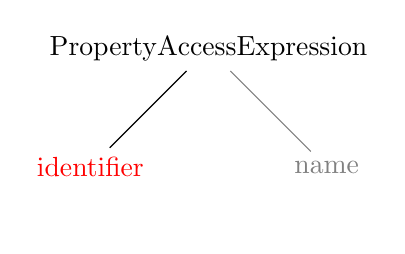
\begin{tikzpicture}
	\node {PropertyAccessExpression}
		child {node [red] {identifier}}
		child [white] {node [yshift = -0.5cm] {\phantom{node}}}  % ensure same height as sibling figures
		child [gray] {node [gray] {name}}
		;
\end{tikzpicture}
\caption[LoF entry]{
	Node pattern for a property access, such as in:

	\code{\lowlight{return }\uline{\lowlight{obj}.\highlight{prop}}\lowlight{;}}
}

			\end{subfigure}
			\hfill
			\begin{subfigure}[t]{.32\linewidth}
				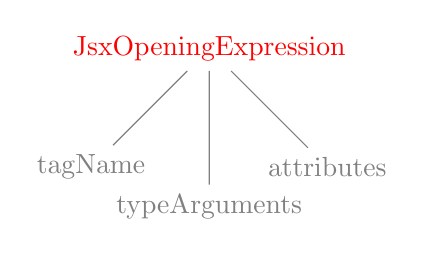
\begin{tikzpicture}
	\node [red] {JsxOpeningExpression}
		child [gray] {node [gray] {tagName}}
		child [gray] {node [gray, yshift = -0.5cm] {typeArguments}}
		child [gray] {node [gray] {attributes}};
\end{tikzpicture}
\caption[LoF entry]{
	Node pattern for a JSX opening element (as supported in React\protect\footnotemark{} or TypeScript\protect\footnotemark{}), such as in:
	\code{\lowlight{elem = }\uline{<Button \lowlight{color}="\lowlight{blue}"> \lowlight{Google</Button>}}\lowlight{;}}
}

			\end{subfigure}

			\caption{AST patterns for example JavaScript/TypeScript expressions.
				The \texthighlight{highlighted} node contains the link to the declaration of the referenced identifier.
			}
			\label{fig:usage_mining/patterns}
		\end{center}
	\end{minipage}
\end{figure*}

Having downloaded the selected downstream dependency repositories, we can proceed to extract usage samples for the target package from each dependency repository.
Our goal is to identify these usage samples on a fine-granular level so that we can trace them down to the single identifiers that were exposed by the target package.

To do so, we start by parsing the source code of every dependency repository as well as the source code of the target package each into a separate abstract syntax forest (ASF, i.e., a set of ASTs).

In a second step, a static type analysis is performed against each dependency ASF together with the target package's ASF.
The results of the type analysis are attached to the ASF so that every identifier is annotated with a type symbol that links to the declaration of the type for the identifier.
For instance, after this step, every variable node will contain a link to the assignment node of this variable, and every function call expression will contain a link to the definition of this function. \TODO{Give example?}
The operating principle of this type analysis depends on the kind of programming language; i.e., in statically typed languages, type symbols can usually be retrieved from the declaration of an identifier, whereas in dynamically typed languages, a control flow analysis will be required to identify the origin of every identifier's type.
\TODO{Elaborate on the topics type analysis and static/dynamic typing in related work/introduction.}

In the final step, from each ASF all nodes are collected whose type is declared in the target package.
To identify these links, we define a set of language-specific patterns for AST subtrees that constitute a usage expression.
In particular, each of these patterns expects a node containing a link to an identifier declaration (see \cref{fig:usage_mining/patterns}).

The complete procedure is displayed in \cref{alg:usage_mining}.

\begin{algorithm}
	\caption{Extraction of usage samples.}\label{alg:usage_mining}

	\KwIn{\\\Indp
		$\mli{pkg}$: target package \\
		$\mli{dependencies}$: downstream dependencies}
	\KwOut{usage samples (set of strings)}
	\;
	\For{$\mli{dep} \in \mli{dependencies}$}{
		$\mli{asf} \gets \mtx{parse}(\mli{dep} \cup \mli{pkg})$\;
	  	$\mtx{annotate\_types}(\mli{asf})$\;
		\For{$\mli{ast} \in \mli{asf}$}{
			\For{$\mli{node} \in \mli{dfs}(\mli{ast})$}{
				\For{$\mli{pattern} \in \mli{patterns}$}{
					\If{$\mli{pattern}.\mtx{matches}(\mli{node}) \wedge \mli{pkg}.\mtx{declares}(\mli{pattern}.\mtx{getType}(\mli{node}))$}{
						\kwYield{$\mli{node}.\mtx{text}$}
					}
				}
			}
		}
	}
\end{algorithm}
